%!TEX root = ../thesis.tex
本章では,オープンプラットフォームのロボットアームの要求仕様を決定していく.行わせる作業を設定し,設定した作業と既存のオフィスロボットの調査を基に要求仕様をまとめていく.
\section{作業の設定}
本研究では,オフィス環境におけるロボットアームの作業として「机の片づけ」を設定した.オフィス環境で想定される作業は多岐にわたるが,基本的には台車移動とピック&プレイス作業を組み合わせたものが大半を占める.これは既存のオフィスロボットがどのような作業を対象にしているかを調査した結果である.文献や動画から78の作業内容を抽出し,そのうち66件(約85%)が台車移動とピック&プレイス作業を組み合わせたものであった.本研究で開発するロボットアームは,将来的にオフィスロボットの標準プラットフォームとなることを期待しているため,最初のステップとして「机の片づけ作業」を設定した.図\ref{fig:range}は,机上における対象物と箱の設置位置を示している.対象物と箱は机の縁から50cm以内の範囲に設置する.また,対象物については既存のオフィスロボットが扱っている物体を調査した結果に基づいて選定した.調査結果を図\ref{fig:handget}に示す.最も多く確認されたのは衣類などの柔軟な物体であり,次いでボトルなどの円柱型物体が多かった.今回はこれらの中からボトルとタオルを対象物として設定した.調査では,重量の大きい物体を把持する作業は確認されず,多くの作業が軽量な物体を対象としていた.これを踏まえ,本研究における対象物の重量を500g以下と設定する.片付け用の箱のサイズは,高さ20cmとする.
\begin{figure}[h]
  \centering
  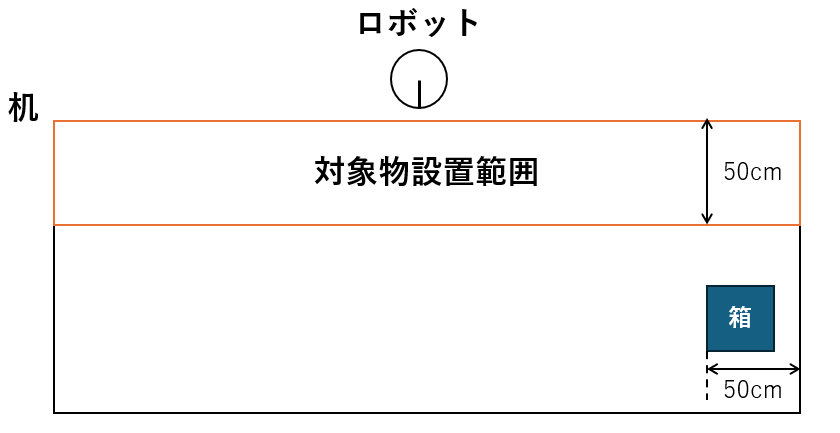
\includegraphics[width=10cm]{images/range.png}
  \caption{Range to place objects and boxes}
  \label{fig:range}
\end{figure}
\begin{figure}[h]
  \centering
  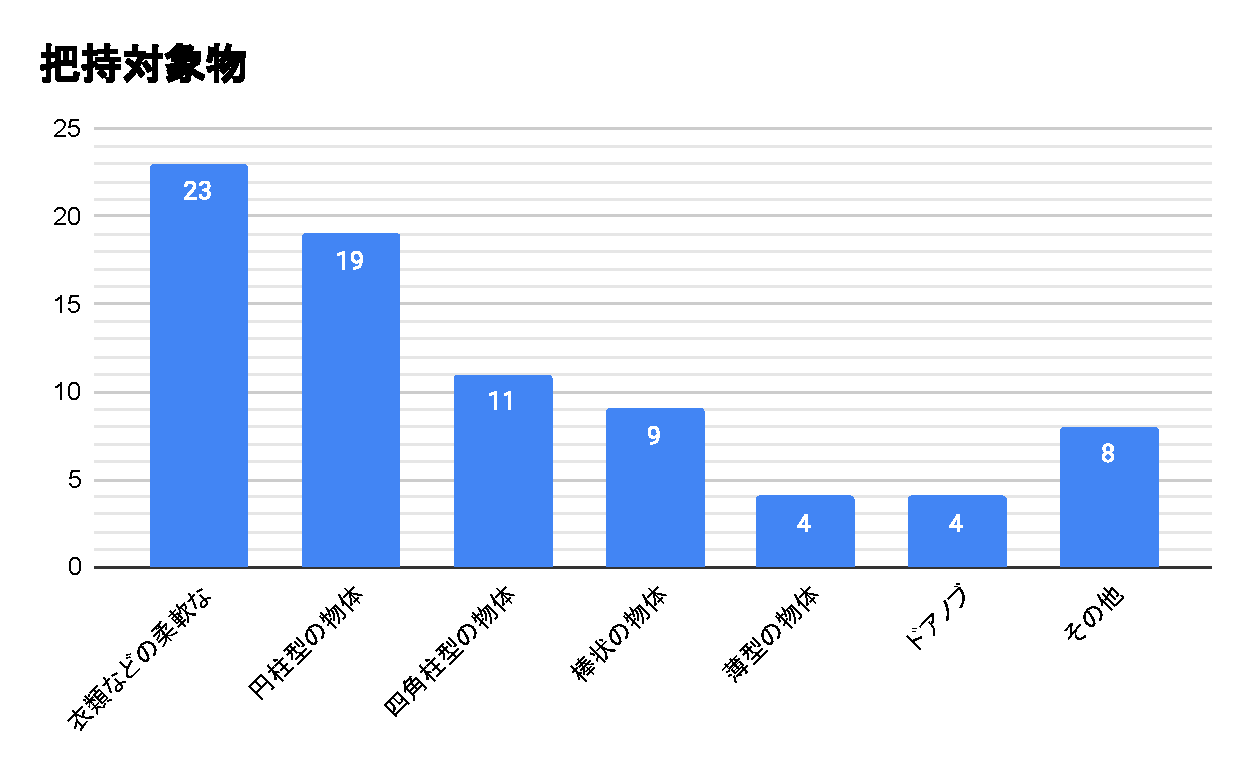
\includegraphics[width=10cm]{images/handget.pdf}
  \caption{Survey results of objects handled by existing office robots}
  \label{fig:handget}
\end{figure}
\clearpage
\newpage